\chapter{Arquitectura del Sistema}\label{cap:08arquitectura}

Este capítulo se divide en cuatro secciones: \ref{sec:08intro} Introducción, \ref{sec:08teorica} Arquitectura teórica del sistema y \ref{sec:08Broadsea} Arquitectura de Broadsea y \ref{sec:08conclusiones} Conclusiones.

\section{Introducción} \label{sec:08intro}

La implementación del ecosistema de herramientas OHDSI y ATLAS puede ser una ardúa tarea. En el contexto de desarrollo del Trabajo Fin de Grado junto a las prácticas en empresa en el Hospital Virgen del Rocío, la dificultad de la tarea se ve exponencialmente aumentada debido a los grandes protocolos de seguridad y privacidad de la administración pública. Por ello, se ha seleccionado el despliegue de las herramientas OHDSI a través del sistema Docker de Broadsea, que presenta una vía sencilla para realizar esta labor. 

Broadsea es un proyecto basado en Docker que permite desplegar todo el entorno de herramientas, configuraciones y dependencias OHDSI de la manera más sencilla hasta el momento. Por tanto, \textbf{el sistema se trata de una virtualización en Docker del entorno de herramientas OHDSI}.

\begin{figure}[H]
    \centering
    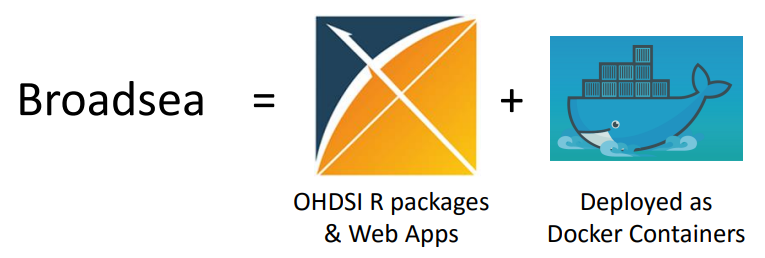
\includegraphics[width=0.70\textwidth]{figures/broadseaEq.png}
    \caption{Esquema sencillo de Broadsea. Extraída de \cite{Broadsea3PPTX}.}
    \label{fig:broadseaEq}
\end{figure}

En la sección \ref{sec:08teorica} ''Arquitectura teórica del sistema'' se presentan los aspectos teóricos fundamentales sobre virtualización y componentes de los sistemas docker y en la sección \ref{sec:08Broadsea} ''Arquitectura tecnológica de Broadsea'' se presenta la arquitectura específica de Broadsea.

No obstante, la arquitectura del sistema también se presenta en mayor profundidad técnica en el Anexo \ref{anexo:manual} ''Manual de instalación, despliegue y configuración de ATLAS Broadsea''.

\section{Arquitectura teórica del sistema} \label{sec:08teorica}

El sistema se implementa mediante virtualización en Docker y una arquitectura en tres niveles o \textit{three-tier}, donde se diferencian al cliente, frontend y backend. Esta arquitectura se describirá de forma general utilizando el esquema de la Figura \ref{fig:threeTierValle}.

\begin{figure}[H]
    \centering
    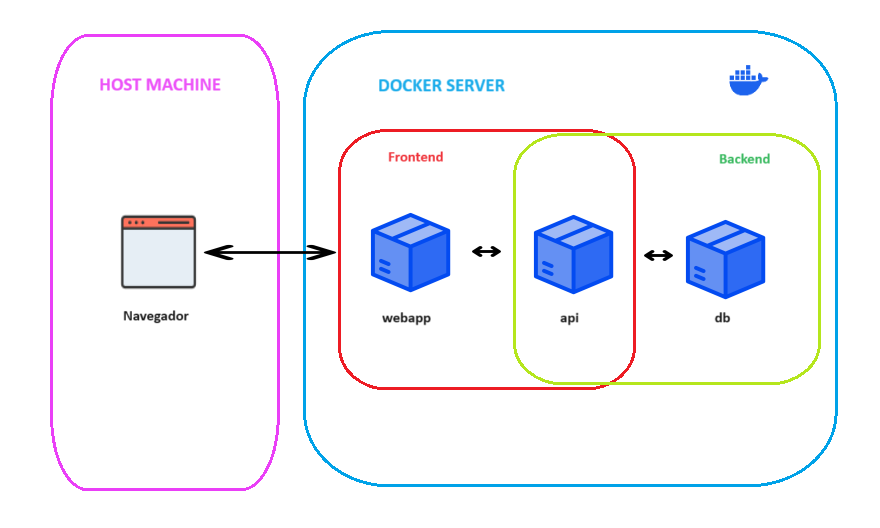
\includegraphics[width=0.80\textwidth]{figures/threeTierValle.png}
    \caption{Esquema de arquitectura \textit{three-tier} en Docker.}
    \label{fig:threeTierValle}
\end{figure}

En primer lugar, la virtualización obliga a diferenciar entre una maquina local o anfitriona (\textit{host machine}, en rosa) y una maquina virtual que provee el servicio docker (\textit{docker service}, en azul). 

\begin{enumerate}

    \item \textbf{La máquina local.} La máquina local es la propia máquina del usuario. Se le denomina anfitriona porque aloja en su interior a la máquina virtual. La máquina local cede un servidor y un puerto a la máquina virtual para que el usuario final pueda acceder al sistema a través de la dirección del servidor en que se aloja, típicamente accediendo mediante un navegador web. El acceso mediante el navegador web es lo que se denomina la capa cliente, pues es la interfaz que permite al usuario acceder al sistema. 

    \item \textbf{La máquina virtual.} La máquina virtual es el sistema virtualizado en Docker. Es el sistema que contiene toda la lógica de la aplicación y los datos empaquetado en un multicontenedor Docker, en este caso el multicontenedor es el propio sistema Broadsea. Está compuesto por tres nodos la \textit{webapp}, la \textit{api} y la \textit{db} que conforman las dos capas restantes de la arquitectura: el frontend y el backend.
    
\end{enumerate}

Por tanto, a nivel de aquitectura del sistema en sí, se encuentra la capa cliente (en el \textit{host machine}, en rosa), el frontend (\textit{network-frontend}, en rojo) y el backend (\textit{network-backend}, en verde).

\begin{enumerate}

    \item \textbf{El cliente.} El cliente está alojado en la máquina anfitriona y proporciona el acceso a los servicios virtualizados del sistema a través de la conexión internet con el servidor docker.

     En el caso de Broadsea el navegador deberá ser Google Chrome y la dirección por defecto será http://127.0.0.1:5432.

    \item \textbf{El frontend.} El frontend está alojado en la máquina virtual, es el servicio que guarda la lógica de la aplicación que se muestra al usuario. Se compone de la \textit{webapp}, que contiene la aplicación como tal, y la \textit{api}. que es la red que permite establecer interconexiones entre la aplicación lógica y la base de datos; entre el frontend y el backend.

    En el caso de Broadsea la webapp y la api se combinan en el componente de la WebAPI, que permite el acceso a la aplicación de ATLAS y maneja las conexión con las bases de datos del backend.

    \item \textbf{El backend.} El backend está alojado en la máquina virtual, es el servicio que aloja la base de datos sobre la que se sostiene la aplicación. Se compone de la \textit{api} y la \textit{db}. De igual forma que en el frontend, la api es la red que permite la interconexión entre los componentes del sistema, en este caso con la base de datos, que puede ser una o varias.

    En el caso de Broadsea, las bases de datos deberán estar estandarizadas a OMOP y podrán encontrarse en el propio servidor Docker, como es el caso de Eunomia, o en servidores externos. No obstante, la relación entre cualquier base de datos y ATLAS se realiza a través de la WebAPI.

    
\end{enumerate}

\section{Arquitectura de Broadsea} \label{sec:08Broadsea}

Broadsea es un sistema muy complejo, contenido en un multicontenedor Docker que alberga el ecosistema completo de herramientas OHDSI y sus interconexiones en distintos contenedores. Además, se definen distintos perfiles (\textit{profiles}) para facilitar la instalación de los distintos contenedores. Por ello se le denomina \textit{a-la-carte}. 

Broadsea es el \textit{docker server} al que se refiere la anterior Figura \ref{fig:threeTierValle} ''Esquema de arquitectura three-tier en Docker''. A continuación se muestran todos los contenedores que alberga el sistema de Broadsea.

\begin{figure}[H]
    \centering
    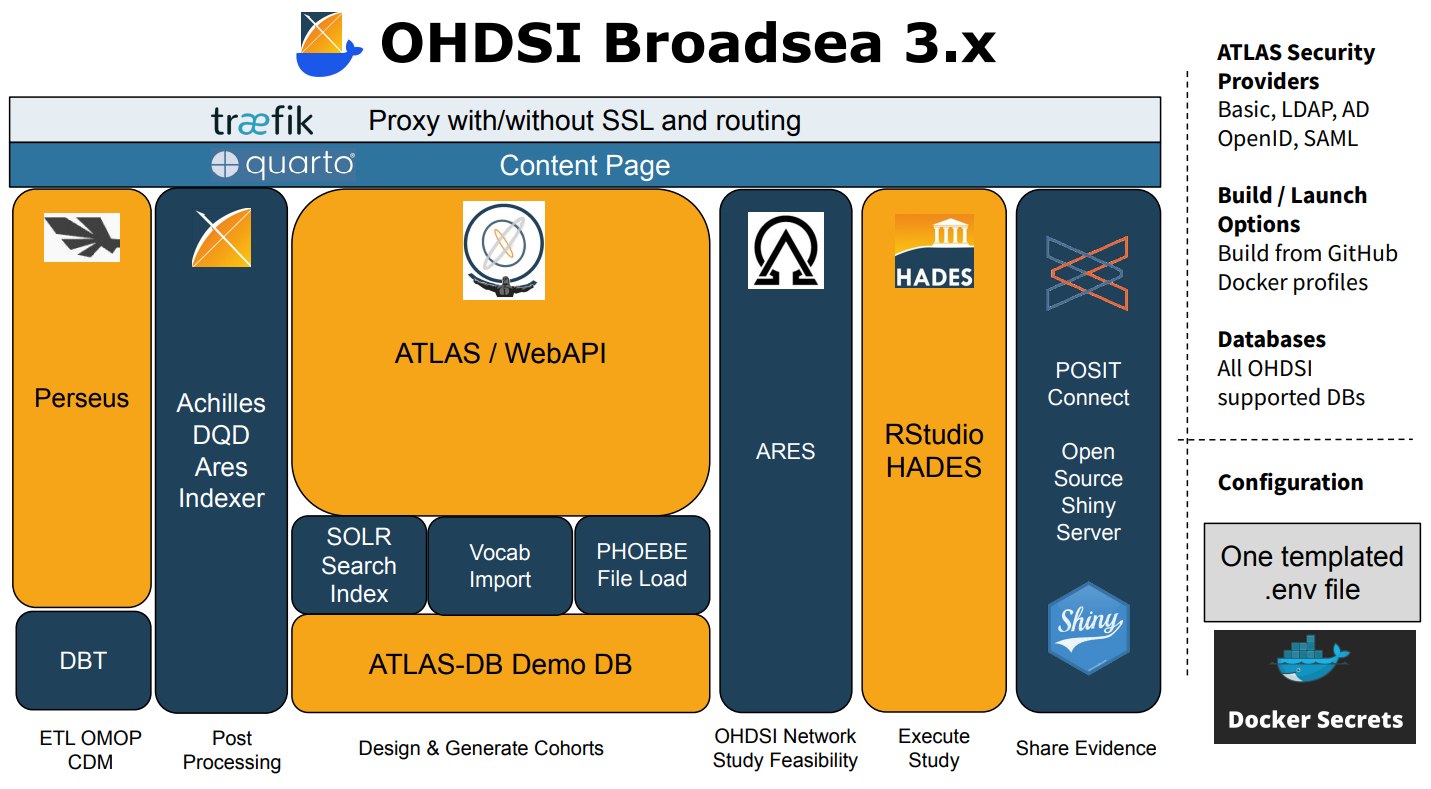
\includegraphics[width=0.90\textwidth]{figures/OHDSIBroadsea3.0.png}
    \caption{Vista general de todos los componentes de Broadsea. Extraída de \cite{Broadsea3PPTX}.}
    \label{fig:OHDSIBroadsea3.0}
\end{figure}

El despliegue por defecto de Broadsea genera una interfaz de usuario con acceso a tres aplicaciones: ATLAS, HADES y ARES. Para acceder a esta interfaz de usuario basta con buscar en el navegador el servidor y puerto donde se aloja broadsea. Tipicamente el servidor corresponde al \textit{localhost} y el puerto 5354, correspondiente a Postgre. La figura a continuación muestra la interfaz principal de herramientas disponibles al acceder a Broadsea desde Chrome.

\begin{figure}[H]
    \centering
    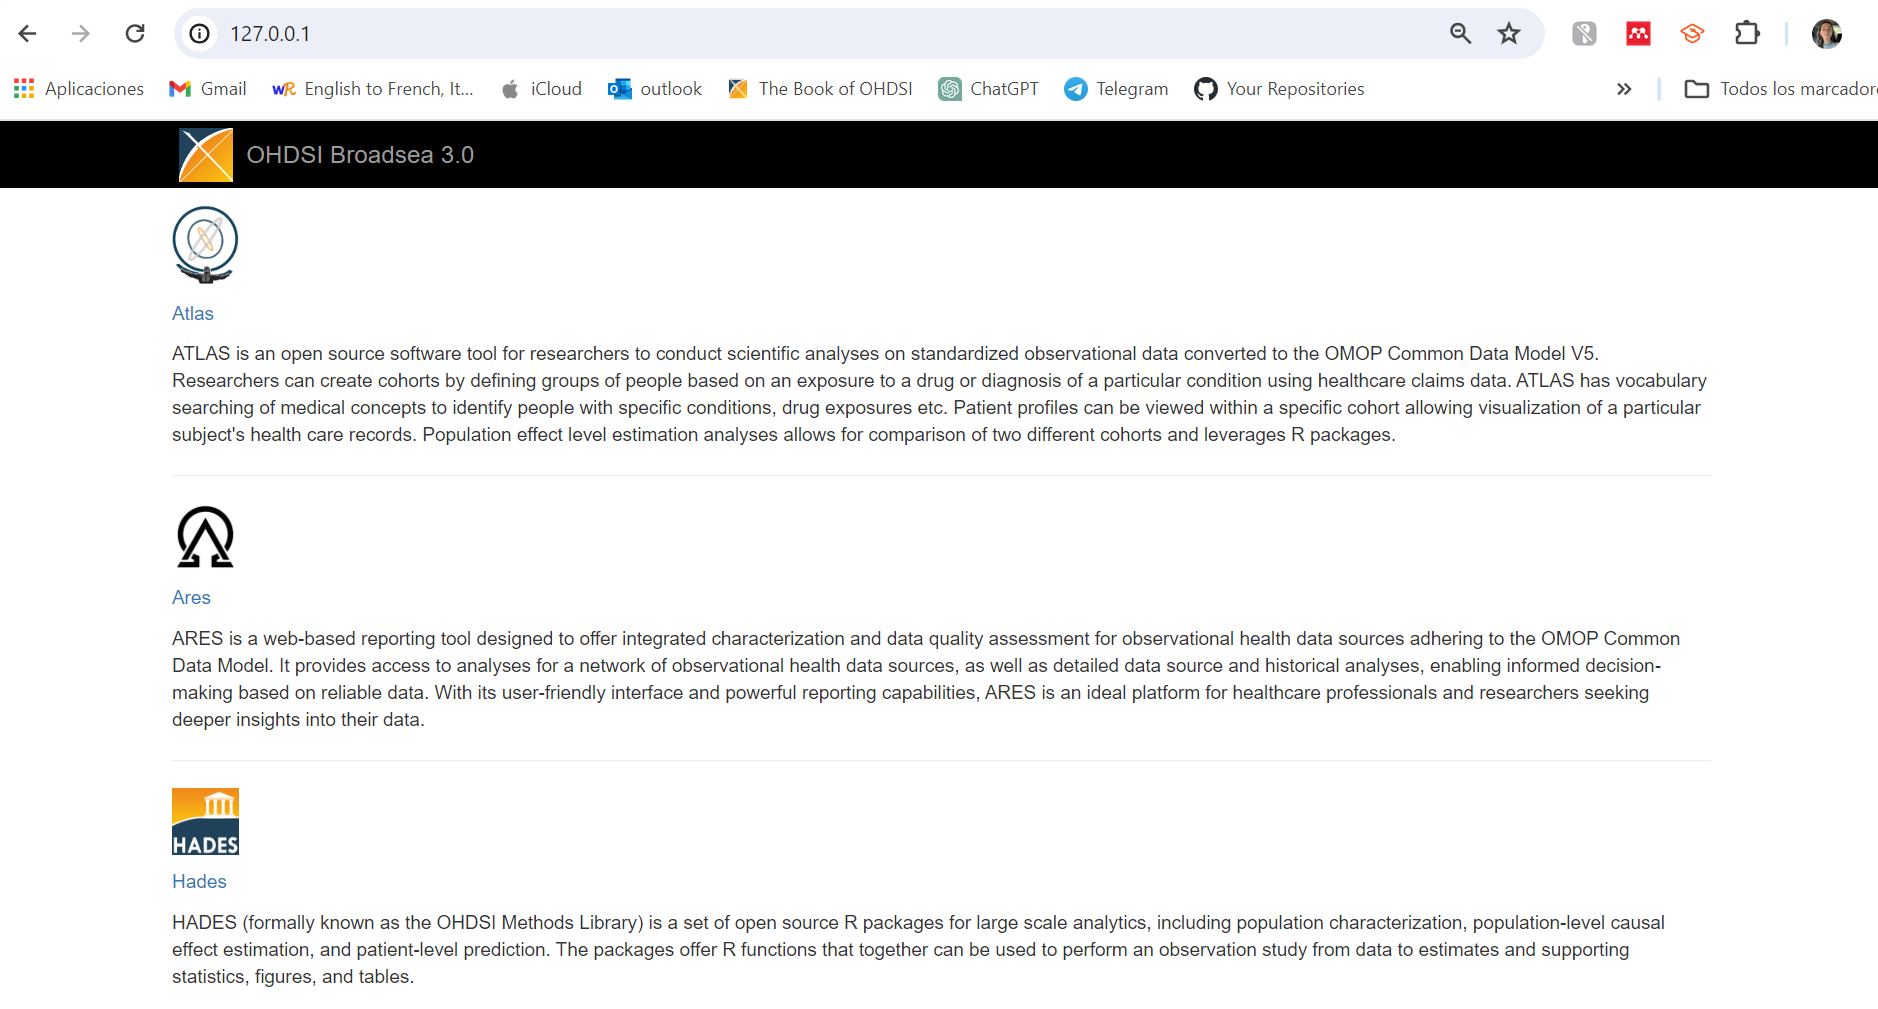
\includegraphics[width=1\textwidth]{figures/homeBroadsea.png}
    \caption{Captura de pantalla del menú principal de Broadsea}
    \label{fig:homeBroadsea}
\end{figure}

Por tanto, haciendo referencia a ambas figuras, se presenta a continuación una breve descripción de cada una de las herramientas accesibles desde el menú principal de Broadsea. En el caso de ATLAS, por su relevancia, se describe la relación de contenedores de Broadsea que participan en su despliegue.

\begin{enumerate}

    \item \textbf{ATLAS}. ATLAS Broadsea despliega todas las funcionalidades de la herramienta de forma local. ATLAS se sostiene sobre la WebAPI y cuenta con la base de datos de Eunomia.
    
    \begin{itemize}
        \item \textbf{WebAPI}. La WebAPI se despliega como un contenedor docker y como un volumen de datos. Además, también se construirá un esquema en la base de datos del servidor Postgre que aloja al contenedor, denominado \code{webapi}. A través de la modificación de este esquema se podrán agregar o eliminar las diferentes fuentes de datos a la herramienta.
        \item \textbf{BD}. Para facilitar el correcto funcionamiento de ATLAS se implementa una base de datos demo que es Eunomia. Esta base de datos cuenta con un pequeño registro de datos normalizados a OMOP y también crea varios esquemas en la base de datos del servidor Postgre que permiten su configuración, o la realización de consultas directamente desde el administrador de la base de datos.
    \end{itemize}

    \item \textbf{HADES}. HADES Broadsea despliega todas las funcionalidades de la herramienta de forma local. Se sostiene sobre una virtualización del IDE de RStudio que tiene preinstalada y preconfiguradas todas las librerías de la Librería de Métodos. Su uso no es relevante en el TFG.
   
    \item \textbf{ARES}. ARES Broadsea despliega todas las funcionalidades de la herramienta de forma local. Su uso tampoco es relevante en el TFG.

\end{enumerate}

\section{Arquitectura de ATLAS Broadsea} \label{sec:08atlas}

ATLAS Broadsea hace referencia a la herramienta ATLAS desplegada a través de Broadsea. Como se ha mencionado previamente, ATLAS Broadsea es accesible a través del navegador Chrome, y se muestra de forma similar a ATLAS demo pero implementada localmente (recuerde Figura \ref{fig:ATLASdemoHome} ''Captura de pantalla del menú principal de ATLAS demo'').  

\begin{figure}[H]
\centering
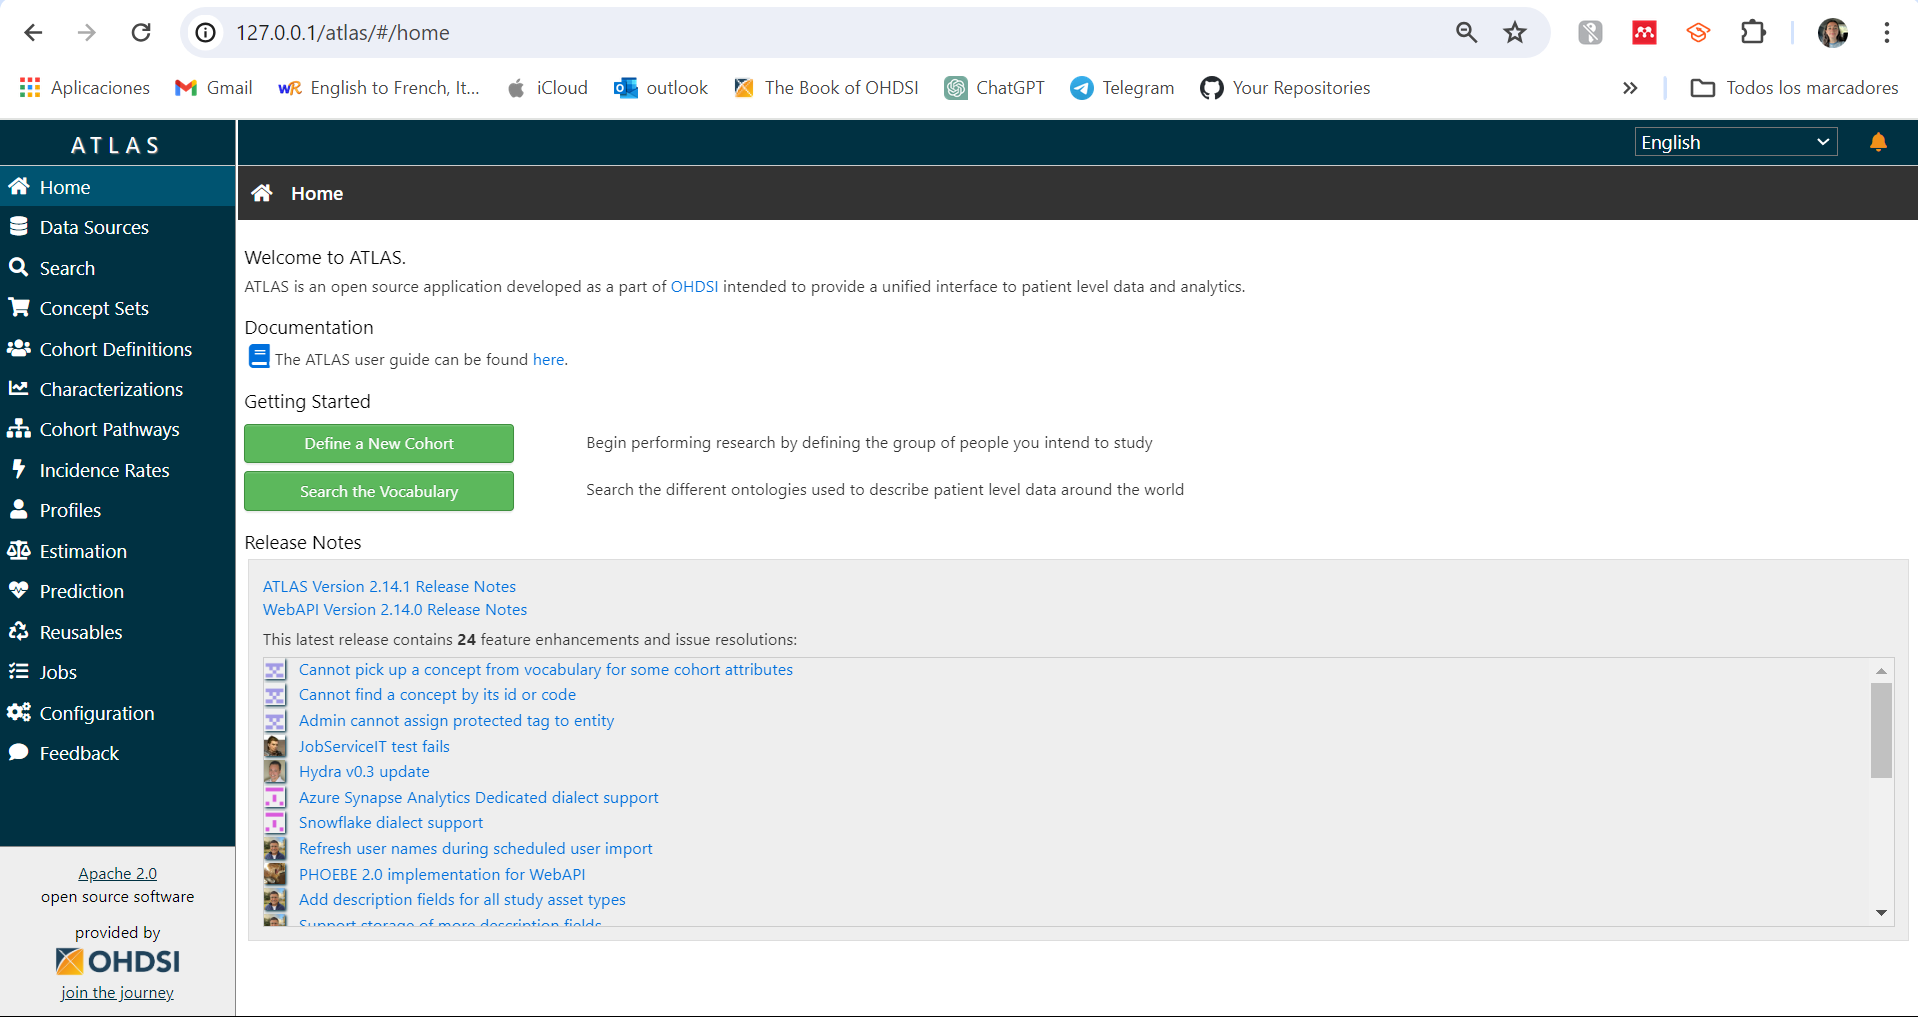
\includegraphics[width=0.90\textwidth]{figures/homeATLAS.png}
     \caption{Captura de pantalla del menú principal de ATLAS Broadsea}
    \label{fig:homeATLAS}
\end{figure}

El menú lateral de ATLAS presenta 15 herramientas de análisis, de las cuales en el proyecto se utilizan las siguientes:

\begin{itemize}
    \item \textbf{Home}. Es el menú principal de ATLAS. Se muestra por defecto al abrir la herramienta.
    \item \textbf{Data Sources}. Es la herramienta para obtener reportes de las bases de datos integradas en la herramienta.
    \item \textbf{Search}. Es la herramienta para realizar búsquedas de conceptos en el Vocabulario.
    \item \textbf{Concept Sets}. Es la herramienta para definir grupos de conceptos que se utilizarán en la realización de análisis.
    \item \textbf{Cohort Definitions}. Es la herramienta para definir las cohortes que intervienen en los estudios y análisis.
    \item \textbf{Characterization}. Es la herramienta para realizar estudios estadísticos de caracterización de las cohortes definidas.
    \item \textbf{Estimation}. Es la herramienta para realizar estudios de estimación a nivel de población.
    \item \textbf{Prediction}. Es la herramienta para realizar estudios de predicción a nivel de paciente.
\end{itemize}

ATLAS Broadsea despliega por defecto la base de datos de Eunomia, que es una pequeña base de datos sintética estructurada al Modelo Común de Datos de OMOP que sirve de ayuda para la toma de contacto con la herramienta. La base de datos de Broadsea es accesible a través de un gestor de bases de datos PostgreSQL como pgAdmin. A continuación se muestra la estructura del servidor y base de datos de Broadsea.

\begin{figure}[H]
\centering
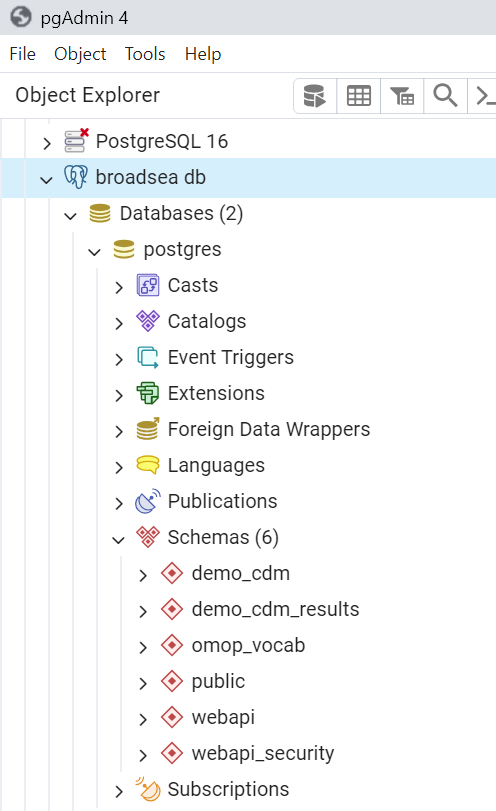
\includegraphics[width=0.60\textwidth]{figures/serverBroadsea.png}
     \caption{Captura de pantalla de pgAdmin de la estructura postgre del servidor de Broadsea}
    \label{fig:serverBroadsea}
\end{figure}

La base de datos presenta seis esquemas, siguiendo la configuración del Modelo de Datos Común de OMOP \cite{githubCDMConfig}. Para mayor información sobre la estructura postgre de Broadsea se recomienda consultar el anexo \ref{anexo:manual} ''Manual de instalación, despliegue y configuración de ATLAS Broadsea''. No obstante, a continuación se describe brevemente la función de cada uno de estos esquemas:

\begin{itemize}
    \item \textbf{demo\_cdm:} Contiene toda la información de eventos clínicos y pacientes registrados en la base de datos. Es el grueso del contenido de la base de datos.
    \item \textbf{demo\_cdm\_results:} Contiene información generada de la ejecución de ACHILLES (véase \ref{sec:07herramientas} ''Herramientas de OHDSI'') sobre la base de datos.
    \item \textbf{omop\_vocab:} Este esquema no venía preinstalado pero es fundamental para el correcto funcionamiento de la herramienta. Contiene todo el vocabulario que va a ejecutar ATLAS. Su intalación se detalla en el manual.
    \item \textbf{public:} Este esquema no pertenece al CDM sino que se genera por defecto al crear una base de datos postgre. No contiene información relevante.
    \item \textbf{webapi:} Es el esquema de la WebAPI. Desde este esquema se establecen y gestionan las conexiones con bases de datos externas.
    \item \textbf{webapi\_security:} Este esquema contiene ajustes para configurar la seguridad de la WebAPI. No se utiliza en el proyecto. Mayor información sobre la seguridad de la WebAPI en el manual.
\end{itemize}


\section{Conclusiones} \label{sec:08conclusiones}

En este capítulo se concluye que la arquitectura tecnológica del sistema es compleja puesto que involucra una virtualización del ecosistema OHDSI a través de Docker, denominado Broadsea. No obstante, la implementación del sistema en Docker facilita bastante la tarea de configurar el ecosistema completo, gracias al empaquetamiento de las funcionalidades en contenedores accesibles \textit{a-la-carte}. 